\documentclass{article}

\usepackage{arxiv}

\usepackage[utf8]{inputenc} % allow utf-8 input
\usepackage[T1]{fontenc}    % use 8-bit T1 fonts
\usepackage{hyperref}       % hyperlinks
\usepackage{url}            % simple URL typesetting
\usepackage{booktabs}       % professional-quality tables
\usepackage{amsfonts}       % blackboard math symbols
\usepackage{nicefrac}       % compact symbols for 1/2, etc.
\usepackage{microtype}      % microtypography
\usepackage{lipsum}
\usepackage{amsmath}
\usepackage{graphicx}
\usepackage{titlesec}
\usepackage{enumitem,kantlipsum}
\graphicspath{{.}}

\title{\textbf{Analysis and Classification of Job Postings as Fake / Legitimate}}

\author{
Amey Meher\\
Department of Computer Science\\ 
North Carolina State University\\
Raleigh, NC 27695 \\
\texttt{avmeher@ncsu.edu}
\And
Abhishek Firodiya \\
Department of Computer Science\\ 
North Carolina State University\\
Raleigh, NC 27695 \\
\texttt{asfirodi@ncsu.edu}
\And
Vaidehi Koppolu       \\
Department of Computer Science\\ 
North Carolina State University\\
Raleigh, NC 27695 \\
\texttt{vkoppol@ncsu.edu}
\And
Chetana Chunduru \\
Department of Computer Science\\ 
North Carolina State University\\
Raleigh, NC 27695 \\
\texttt{cchetan2@ncsu.edu}
}
\date{} % clear date

\titlespacing*{\subsubsection}
{0pt}{.2ex}{.2ex}

\begin{document}
    \renewcommand{\labelenumii}{\arabic{enumi}.\arabic{enumii}}
    \renewcommand{\labelenumiii}{\arabic{enumi}.\arabic{enumii}.\arabic{enumiii}}
    \renewcommand{\labelenumiv}{\arabic{enumi}.\arabic{enumii}.\arabic{enumiii}.\arabic{enumiv}}
    \renewcommand{\labelitemi}{$\bullet$}
    \renewcommand{\labelitemi}{$\bullet.\bullet$}

    \maketitle

    \vspace{-30pt}
    \begin{center}
        \textbf{Group P12}
    \end{center}

    \begin{enumerate}[wide, labelwidth=!, labelindent=0pt]
        \item \textbf{Introduction}\\\\
        In this time of impending recession in the IT sector, the number of cases of fraudulent job posting is increasing. According to the Federal Trade Commission, Americans were scammed out of \$68 million in the first quarter of 2022 due to fraudulent business and job opportunities. Employment-related scams have been a persistent problem, but they increased in 2020 as criminals preyed on people who had lost their jobs due to Covid. Employment scams have only become more sophisticated, so it's critical to be cautious as a job seeker. For addressing this issue, our project aims to leverage the power of Machine Learning models to predict the genuineness of Job postings based on history data. \\

        \item \textbf{Background}\\\\
        Classification is a technique for categorizing data into a set number of groups. Its main goal is to determine which category/class a new data set belongs to. A classification model attempts to derive some conclusion from the training input values. It will predict the new data class labels/categories. Classification can be used to perform a wide range of tasks, including speech recognition, handwriting recognition, biometric identification, document classification, and so on.\\\\
        Our project's goal is to be able to classify job postings as legitimate or not based on the data attribtes used to train the model. Because we have the output label for the data points, this falls under the Supervised Machine Learning use case, and for our project, we are using classification models such as Decision Tree, K Nearest Neighbours, Bayes Classifier, etc. In addition, we hope to discover valuable patterns in the data by using various visualization techniques to gain a better understanding of the data.\\\\

        \item \textbf{Method}
        \begin{enumerate}
            \item \textbf{Data Selection}\\\\
            The dataset for this project can be found at the link: \href{https://www.kaggle.com/datasets/shivamb/real-or-fake-fake-jobposting-prediction}{https://www.kaggle.com/datasets/shivamb/real-or-fake-fake-jobposting-prediction}. The dataset consists of 17880 data points, of which 866 are classified as fake job postings under the 'fraudulent' attribute. It also consists of data elements such as job title, location of work, department of the job role, salary range and other metadata related to job profile. We are removing Job IDs as they do not contribute in any decision making process. The dataset also contains NULL elements in some of the attributes as well as duplicate entries - for which proper cleaning technique is applied.\\

            \item \textbf{Data Pre-processing}\\\\
            The dataset used in this project has a lot of null, 'Not Applicable' and 'Unsatisfied' values. We are replacing those values with value 'No Info' because all three of these values are corresponding to same thing. We are removing 282 duplicate rows from dataset which reduces its size to 17598.
            Also, the dataset is poorly balanced. Most jobs are legitimate, with only a few exceptions. Data points are being classified as genuine or legitimate due to this when we analysed the accuracy of our models. We are therefore exploring SMOTE which can be used to generate synthetic minority class samples. A well-balanced dataset would yield better results.\\

            \item \textbf{Data Transformation}\\\\
            There are 11 string attributes for which transformation is done to collect valuable information out of it. These categorical datapoints are converted to numeric datapoints to ease the data mining.
            For the next part, the numeric / categorical part of the dataset will be converted to a different base system using Principal Component Analysis (PCA), which will help us extract only the dimensions along which the variance is the maximum. This would reduce the training overhead for the model and will result in lesser amount of time required for testing and evaluating multiple models.We are also exploring the use of Linear Discriminant Analysis (LDA) technique for the dimensionality reduction. We’ll be comparing the performance based on these both and if possible, would devise our approach as per the results.\\

            \item \textbf{Data Mining}\\\\
            We are planning to evaluate the below classifiers for our problem statement--
            \begin{itemize}
                \item K- Nearest Neighbors (KNN)
                \item Decision Tree
                \item Support Vector Machine (SVM)
                \item Naive Bayes Classifier
            \end{itemize}
            Currently, we have trained different KNN models based on varying values of K and evaluated their performance.
            The models would be evaluated based on results from Cross Validation for the value of k=10.\\\\

            \item \textbf{Interpretation and Evaluation}\\\\
            There are different metrics upon which we can evaluate the performance of our models. Metrics such as Recall / Sensitivity, Precision, F1 Score etc can be utilized. We are specifically focusing on the Sensitivity metrics for evaluation.\\\\
            The Sensitivity value of a machine learning model is a measure of its ability to detect positive instances. It's also referred to as the true positive rate (TPR) or recall. Sensitivity is used to assess model performance because it shows how many positive instances the model correctly identified. A model with high sensitivity will have few false negatives, implying that it will miss some positive instances. In other words, sensitivity assesses a model's ability to correctly identify positive examples. This is significant because we want our models to be able to detect all positive instances in order to make accurate predictions.\\\\
            For our project, we have assumed the positive scenario to be a prediction for legitimate job posting and a negative job posting as Fraudulent. The scenario of having a False negative, i.e. predicting a job to be genuine whereas in actual it was fraudulent would carry a higher cost as it would have a critical impact on the applicant in terms of monetary status. Since, Sensitivity focuses on reducing the false negatives in the system, we are using this metric for evaluating the models.\\\\
        \end{enumerate}

        \item \textbf{Experiment Setup}\\\\
        We have implemented the code using the packages such as sklearn for model related functionalities, numpy and pandas for data manipulation, seaborn and matplotlib for data visualization. For collaboration purposes, we have used Git and Google Collab so as to work on the project in a distributed manner.\\\\
        Currently, we have progressed with the K-Nearest Neighbor (KNN) classifier. We have created 4 different models for this classifier and below are the metrics that we have chosen for training the KNN classifiers--
        \begin{itemize}
            \item Distance metric: Euclidean distance
            \item k values: 1,3,5,9
            \item Training and testing division: 80:20
        \end{itemize}
        % \vspace{-1cm}
        For the later part of project, we aim to implement cross validation for the above KNN models to choose the best model with the optimal k value. We aim to implement a generic flow for cross validation so as to be utilized for other classifiers as well, which would reduce code overhead.

        \item \textbf{Results}\\\\
        After experimenting, we got following test results--
        \begin{itemize}
            \item The dataset has 17880 datapoints, of which 866 are classified as fake job postings under the 'fraudulent' attribute.
            \item The dataset has total of 70103 null values and 282 duplicate rows.
            \item The unique counts for each column in the dataset as well as unbalanced data for label 'fraudulent' are visualized.
            \hspace*{-2cm}
            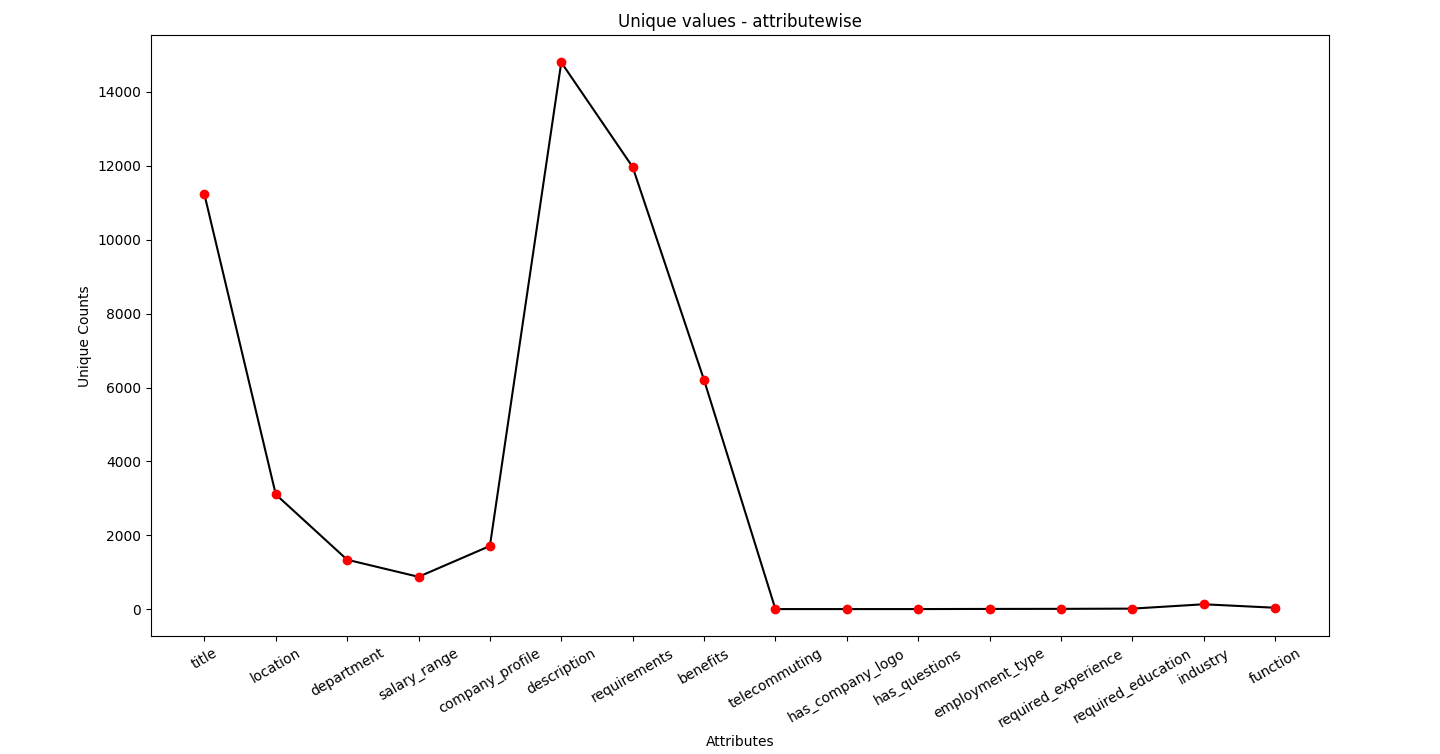
\includegraphics[width=20cm, height=10cm]{images/1.data_select.png}
            \begin{center}
            \caption{Figure 1: Unique values in the dataset}
            \end{center}\\\\

            \hspace*{1cm}
            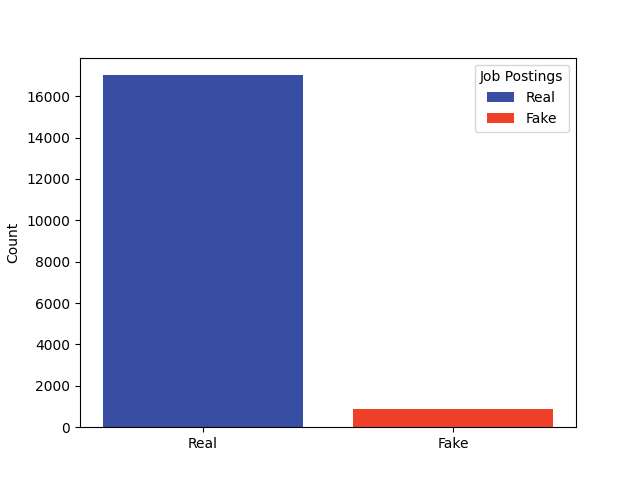
\includegraphics[width=15cm, height=10cm]{images/2.unbalanced_data.png}
            \begin{center}
            \caption{Figure 2: Unique values in the dataset}
            \end{center}\\\\
            
            \item Heatmap is used to find correlation between all attributes.\\
            \hspace*{-2cm}
            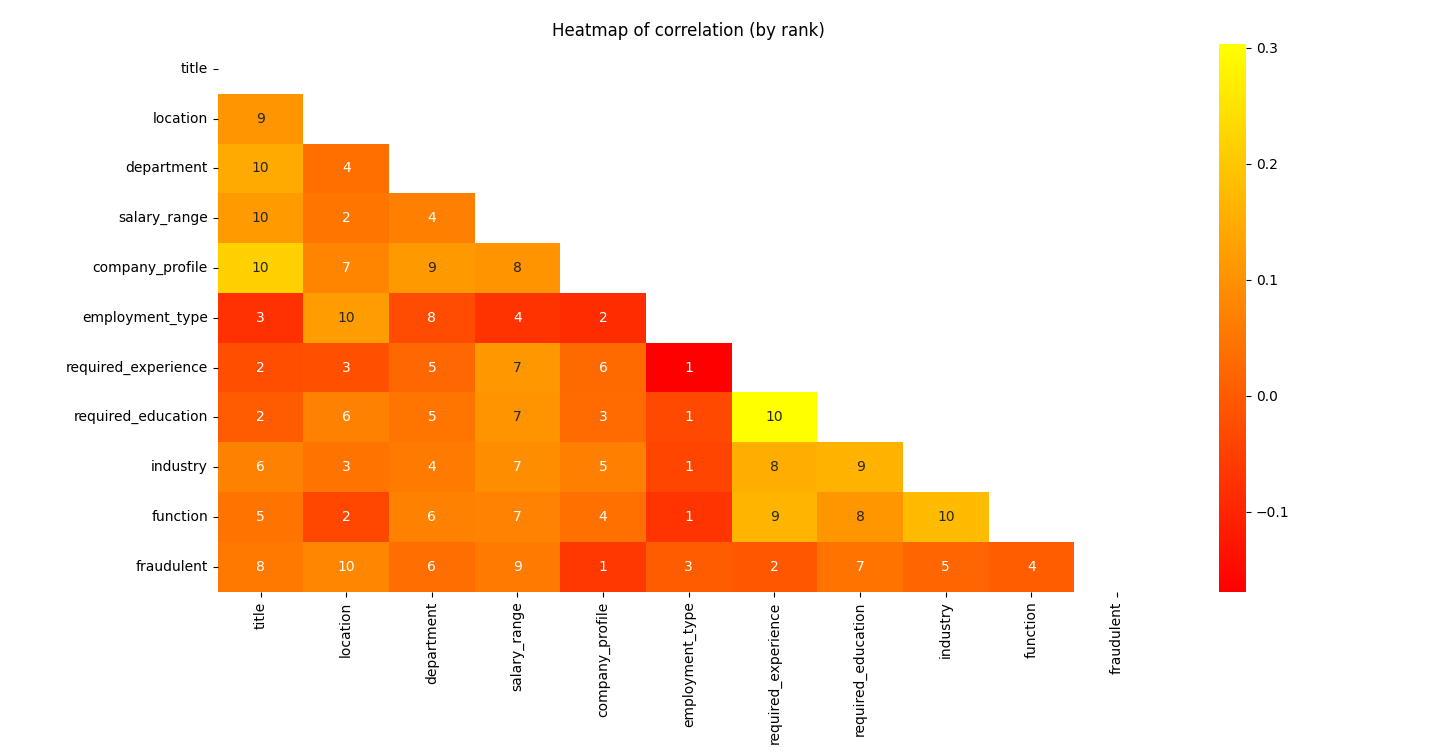
\includegraphics[width=20cm, height=10cm]{images/3.heatmap.png}
            \begin{center}
            \caption{Figure 3: Heatmap of correlations}
            \end{center}\\\\
            
            \item  \textbf{KNN Model}\\\\
            We have listed the accuracy, recall and precision of KNN for different values of k (1, 3, 5, 9)\\
            \hspace{2cm}
            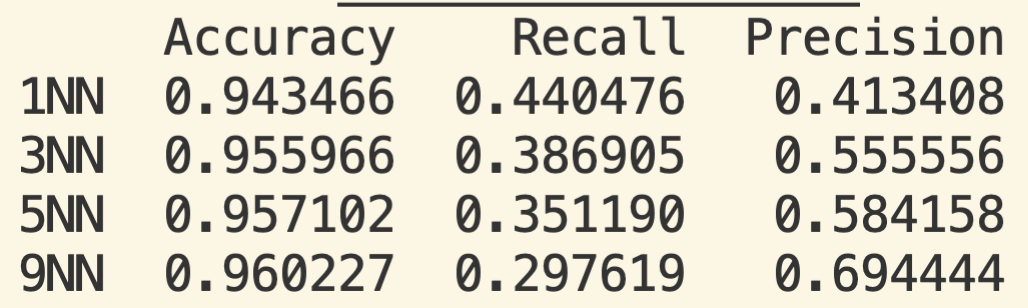
\includegraphics[width=10cm, height=3cm]{images/4.knn_cm.png}
            \begin{center}
            \caption{Figure 4: Evaluation Metrics for KNN}
            \end{center}
        \end{itemize}\\


        \item \textbf{Conclusion}\\\\
        The real and fake job posting project taken was selected to solve a real world challenging issue. This project aims to provide solution to this problem. The dataset taken from kaggle has been pre-processed and pertinent columns have been selected based on the resultant data plots. The null values throughout the data have been generalised to a common value to maintain standardisation. The duplicates in the data set have been removed to have a clean data. Correlation has been used to give the relation between different features and this coupled with a heatmap is used to identify the relevant features which are highly related to the class label. The dataset is then splitted into train, test and validation sets to be used in the classification models.\\\\ 
        Currently KNN Classification model has been used to fetch the model evaluation metrics where it resulted in high frequencies which makes it an overfitting model.To address this issue we will try to implement Synthetic Minority Oversampling Technique (SMOTE) and try to resolve the imbalance problem. The future scope is to identify the best classification model for the dataset and predict the real and fake jobs which will be delivered as part of the final report.\\\\

    \end{enumerate}

\end{document}